\chapter{Revisão Bibliográfica} \label{chap:sota}

\section*{}

%Neste capítulo é feita a descrição do estado da arte e são também apresentados 
%Neste capítulo é descrito o estado da arte e são
%apresentados trabalhos relacionados para mostrar o que existe no
%mesmo domínio e quais os problemas em aberto.
%Deve deixar claro que existe uma oportunidade de desenvolvimento que
%cobre alguma falha concreta .
%
%O capítulo deve também efetuar uma revisão tecnológica às principais
%ferramentas utilizáveis no âmbito do projeto, justificando futuras
%escolhas.

\section{Introdução}

Neste capítulo é ilustrada a utilização de dispositivos móveis para efeitos de pagamento e validação ou ativação de serviços. São também apresentados alguns projetos já implementados em diversas áreas que tiram proveito dos dispositivos móveis para proporcionar ao utilizador uma alternativa mais cómoda para realizar as referidas operações.
\\Dado o enorme crescimento de ativação de dispositivos móveis e a respetiva queda de preços, é cada vez maior o número de aplicações existentes no mercado, cobrindo uma variedade de áreas de negócio cada vez mais vasta. Estas aplicações utilizam tecnologias diferentes e, como tal, neste capítulo são exploradas as mais pertinentes, no âmbito do projeto.

\section{Pagamentos Móveis}\label{sec:pagmov}

Os pagamentos móveis e outros serviços móveis, como por exemplo \textit{mobile banking}, originalmente eram baseados em mensagens de texto para completar as transações. O primeiro exemplo de pagamento móvel surgiu em 1997 quando a Coca Cola introduziu um número limitado de máquinas de venda, em Helsínquia, Finlândia, onde o cliente poderia efetuar um pagamento móvel. O cliente enviaria uma mensagem de texto para a máquina de venda para configurar o pagamento e a máquina venderia então o produto. \textit{Mobile banking} surgiu também em 1997, através do banco finlandês Merita, e aceitava mensagens de texto para realizar transações na conta bancária.\cite{nfcorg}
\\Os serviços relacionados com comércio móvel aumentaram rapidamente no início do século XXI. A Noruega lançou pagamentos móveis de estacionamento, a Áustria, compra de bilhetes de comboio através de dispositivos móveis e no Japão surgiu a compra de bilhetes de avião.
\\Desde então muitos têm sido os desenvolvimentos na área dos pagamentos móveis e as empresas veem neles uma mais valia para os seus produtos, tornando mais fácil a venda de serviços aos seus clientes. Apesar de ainda se continuar a usar SMS para efetuar transações, surgiram outras tecnologias com mais funcionalidades e segurança acrescida. Hoje em dia são vários os produtos que se baseiam em USSD, débito direto, WAP, QR Code, e NFC.

\subsection{Pagamentos via SMS/USSD} \label{smsussd} 

O cliente envia um pedido de pagamento através de uma mensagem de texto SMS ou USSD para um \textit{short code} e é aplicado um débito no seu saldo do telemóvel ou numa carteira virtual. O vendedor é informado do sucesso da operação e envia então o conteúdo desejado.\cite{Blervaque2003} Como normalmente não há um endereço de entrega fiável definido, estes conteúdos são normalmente digitais, sendo a resposta recebida através de MMS contendo o conteúdo comprado (músicas, toques, fundos, etc.). Podem ser também enviados códigos de barras através de MMS que servem depois para confirmar o pagamento por parte do vendedor. Este método é utilizado como um bilhete eletrónico para aceder ao cinema ou eventos ou para recolha de objetos físicos.
\\Este meio de pagamento está a ser cada vez mais substituído pelos que se apresentam posteriormente, sendo as principais razões as que se seguem:
\begin{itemize}
\item Pouca fiabilidade – As transações podem facilmente falhar, tendo em conta que as mensagens se podem perder;
\item Velocidade baixa – Enviar mensagens pode ser um processo lento e pode levar horas até o vendedor receber a confirmação do pagamento. Os clientes não querem ter de esperar mais do que alguns segundos;
\item Segurança – A encriptação de SMS/USSD termina na interface de rede, portanto a mensagem é texto puro, sem qualquer encriptação;
\item Custo elevado – Há muitos custos associados a este tipo de pagamento. Primeiro o custo de definir um \textit{short code}, depois o custo de enviar os conteúdos para os clientes através de MMS e também os custos de apoio ao cliente para os casos de mensagens perdidas ou atrasadas.
\end{itemize} 
Alguns serviços de pagamento móvel aceitam "pagamentos SMS Premium"\cite{mobile}. O processo é o seguinte:
\begin{enumerate}
\item Cliente envia SMS com código do serviço e número único para um \textit{short code};
\item Cliente recebe um PIN (o débito é efetuado aquando da receção do PIN);
\item Cliente utiliza o PIN para aceder a conteúdos ou serviços.
\end{enumerate}

\subsection{Pagamentos via débito direto} \label{direto}

O cliente usa a opção de débito móvel durante a compra numa página \web de comércio eletrónico (por exemplo, uma página de jogos online) para efetuar o pagamento. Depois de uma validação em dois passos, envolvendo um PIN e uma OTP (\textit{One Time Password}), o débito é efetuado no saldo móvel do cliente. É um método de pagamento que não exige o uso de cartões de crédito ou débito nem o registo numa solução de pagamento online tal como a PayPal, saltando assim a intermediação por parte de bancos ou empresas de cartões.\cite{dmb} Este tipo de pagamento é extremamente predominante e popular na Ásia, caracterizando-se pelos seguintes atributos:
\begin{itemize}
\item Segurança – A autenticação em dois passos e um motor de gestão de risco previne fraude;
\item Conveniência – Não é necessário pré-registo nem aplicação móvel específica;
\item Facilidade – Trata-se de apenas uma nova opção durante o processo de pagamento numa compra;
\item Rapidez – A maioria das transações é completa em menos de dez segundos.
\end{itemize}

\subsection{Pagamentos via WAP} \label{wap} 

O cliente usa uma página \web ou uma aplicação instalada no telemóvel para fazer o pagamento. Usa o WAP como tecnologia base e portanto herda todas as suas vantagens e desvantagens. As vantagens incluem:
\begin{itemize}
\item Possibilidade de encaminhar o cliente para outra página após a transação, por exemplo a página da loja ou outros produtos que o cliente possa gostar. Essas páginas têm um URL que pode facilmente ser adicionado aos marcadores e revisitado mais tarde ou partilhado;
\item Elevada satisfação dos clientes por pagamentos rápidos e previsíveis;
\item Facilidade de uso a partir de um conjunto familiar de páginas de pagamento.
\end{itemize}
No entanto, a não ser que seja utilizado débito direto por parte da operadora móvel, há necessidade de usar um cartão de crédito ou débito ou o registo numa solução de pagamento online, tal como numa transação feita através do computador.

\subsubsection{Débito direto pela operadora}

Débito direto pela operadora, também conhecido como débito WAP, requer integração com a operadora. Isso traz alguns benefícios, nomeadamente o facto de as operadoras já terem uma relação de débito com os clientes, bastando adicionar o pagamento à conta do cliente. Para além disso, permite realizar pagamentos instantâneos e proteger os detalhes do pagamento e a identidade do cliente. Uma outra vantagem é o facto de se poder reduzir os custos de apoio ao cliente por parte dos vendedores.
\\A principal desvantagem é que os lucros são normalmente menores do que usando um outro fornecedor de pagamentos.
\\Em 2012, a Ericsson e a Western Union aliaram-se para expandir o mercado de débito direto pela operadora, tornando possível às operadoras móveis incluir transferências de dinheiro móveis Western Union como parte do seu serviço financeiro móvel. Dada a visibilidade internacional de ambas as companhias, esta parceria provavelmente irá acelerar a interconexão entre o comércio móvel o mundo financeiro existente.\cite{ericsson}

\subsubsection{Cartão de crédito/débito}
Um sistema de pagamento \web pode também incluir um formulário de pagamento através de cartão de crédito ou débito, permitindo ao cliente inserir os dados do cartão para efetuar pagamentos. Este processo é familiar, mas a introdução de quaisquer detalhes num telemóvel é mais suscetível a erros e consequentemente a falhas no pagamento. Para além disso, um vendedor pode automaticamente e de forma segura associar os detalhes do cartão ao cliente e, em futuras compras, permitir ao utilizador que realize o pagamento através de um simples clique, removendo assim o fator de erro associado à introdução manual dos detalhes do cartão.

\subsubsection{Carteiras virtuais}
Companhias como a PayPal, Amazon ou Google também fornecem opções de pagamento móvel. Normalmente o processo baseia-se no registo por parte do utilizador, introduzindo o seu número de telemóvel. Posteriormente recebe um PIN por SMS e autentica o seu número de telemóvel através desse PIN. De seguida, o utilizador introduz os dados do cartão de crédito ou outro meio de pagamento (se necessário) e valida o pagamento. Nos pagamentos seguintes, será apenas necessário introduzir o PIN para autenticar e validar o pagamento.

\subsection{Pagamentos via QR Code} \label{qrcode} 

Desde novembro de 2012 que são utilizados pagamentos via QR Code em grande escala na República Checa, sob a forma de um formato aberto de troca de informação de pagamentos, \textit{Short Payment Descriptor}.\cite{qrplatba} 
\\O \textit{Short Payment Descriptor} (SPAYD) usa a estrutura de um \textit{vCard} e a semântica de um pagamento SEPA. Está desenhado para ser compacto, legível e, portanto, fácil de implementar. O formato permite extensões usando atributos com o prefixo "X-".
\\Exemplo de conteúdo de um SPAYD e respetivo QR Code na Figura~\ref{fig:spayd}: 
\\SPD*1.0*ACC:CZ1355000000000000222885*AM:250.00*CC:CZK*MSG:FOND HUMANITY CCK*X-VS:333

\begin{figure}[t]
  \begin{center}
    \leavevmode
    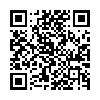
\includegraphics{spayd}
    \caption{SPAYD armazenado num QR Code}
    \label{fig:spayd}
  \end{center}
\end{figure}

\subsection{Pagamentos via NFC} \label{nfc} 

\textit{Near Field Communication} (NFC) é usada maioritariamente para compras feitas em lojas físicas ou serviços de transportes. Um cliente, usando um telemóvel especial equipado com um \textit{smartcard} aproxima o dispositivo de um módulo de leitura. A maioria das transações não requer autenticação, mas algumas fazem-nos através de PIN, antes de completar a transação. O pagamento pode ser deduzido duma conta pré-carregada ou debitada diretamente do saldo do telemóvel ou de uma conta bancária.\cite{SmartCardAlliance2011}
\\Pagamentos móveis através de NFC enfrentam desafios significativos para uma rápida e abrangente adoção, devido à falta de infraestruturas de suporte, ao complexo ecossistema de intervenientes e standards. Apesar disso, alguns produtores de telemóveis e bancos estão entusiasmados com esta tecnologia emergente.\cite{vdc}
\\Os fornecedores de NFC no Japão estão intimamente ligados a redes de trânsito massivo, como por exemplo a Mobile Suica, utilizado na rede férrea JR East. O sistema Osaifu-Keitai, utilizado na Mobile Suica e em muitas outras aplicações, tornou-se o método standard para pagamentos no Japão.
\\Outros fornecedores, principalmente na Europa, usam pagamentos sem contacto através de telemóveis para estacionamento em parques ou na rua em áreas especialmente demarcadas. Os clientes beneficiam porque podem fazer o pagamento no conforto do seu carro com o seu telemóvel e os operadores de estacionamento não são obrigados a investir em infraestruturas, novas ou existentes. Os responsáveis pelo estacionamento mantêm a ordem através da matrícula, \textit{transponders} ou códigos de barras.
\\Alguns fornecedores usam uma combinação de NFC e código de barras no dispositivo para pagamento, tornando esta técnica mais atrativa nos pontos de venda porque muitos dispositivos móveis no mercado ainda não suportam NFC.\cite{cimbal}

\section{Projetos} \label{projetos}

\subsection{MB Phone}

Lançado em 1996, o MB Phone é um serviço inovador que permite efetuar no telemóvel algumas das operações que, habitualmente, se efetuam no Caixa Automático (normalmente conhecido por multibanco ou ATM). Estas operações têm a particularidade de poderem ser realizadas com ecrãs idênticos aos encontrados nos Caixa Automático, através de uma aplicação Java. Pode ainda utilizar-se o serviço através de serviços de voz ou SMS. 
\\O serviço MB Phone está ativo 24 horas por dia, em Portugal ou em qualquer outro país, com o qual a operadora de telecomunicações tenha acordos de roaming.
\\Ao aliar a mobilidade à funcionalidade, este serviço vai ao encontro do consumidor final mas também dos bancos acionistas que apresentam um serviço que satisfaz as necessidades dos seus clientes. Este serviço está disponível nas operadoras TMN, Vodafone e Optimus e permite as seguintes operações: carregamentos de telemóveis (pré-pagos), pagamentos de serviços, consultas de saldos e movimentos bancários, consultas de NIB, pedidos de livros de cheques e transferência entre contas associadas.\cite{mbphone}
\\A utilização do MB Phone pode ser feita de três maneiras distintas:
\begin{itemize}
\item Aplicação Java – Esta aplicação simula no seu telemóvel os menus de um Caixa Automático;
\item Chamada telefónica – As instruções são dadas durante a chamada;
\item SMS – A mensagem SMS é composta pelos seguintes campos [telecódigo] [cód. da operação] [n.º de seq. da conta] [outros].
\end{itemize}

\begin{figure}[t]
  \begin{center}
    \leavevmode
    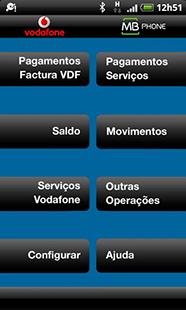
\includegraphics{mbphone}
    \caption{Menu Principal da Aplicação MB Phone para Android}
    \label{fig:mbphone}
  \end{center}
\end{figure}

%%%%%%%%%%%%%%%%%%%%%%%%%%%NEEDS CONFIRMATION
\subsection{WalletPT} 

O WalletPT é uma solução inovadora que permite fazer pagamentos em edifícios PT através do telemóvel. Este serviço baseia-se num saldo pré-pago, distinto do saldo de comunicações, que pode carregar-se na página \web através de diversos meios de pagamento, nomeadamente cartão de crédito, PayPal, multibanco ou MB Phone. É este saldo que permite efetuar pagamentos nos vários comerciantes aderentes. Desta forma, é possível controlar eficazmente os gastos, podendo consultar-se todo o histórico de movimentos na página \web ou os mais recentes através do telemóvel. Pode ser efetuada qualquer compra mesmo sem ter dinheiro na carteira.
\\Para se utilizar o serviço é necessário um registo prévio e estão disponíveis quatro formas de pagamento:
\begin{itemize}
\item SMS
\subitem Enviar SMS grátis para o 5665 com "pagar" e será enviado uma mensagem SMS com um código para o telemóvel;
\subitem No ecrã do terminal de pagamento escolher SMS;
\subitem Inserir no terminal de pagamento o código recebido por SMS;
\subitem Selecionar o produto pretendido.
\item USSD
\subitem No ecrã do terminal de pagamento escolher USSD;
\subitem Marcar, no telemóvel, o número indicado no ecrã (*\#566*código*pin de segurança\#);
\subitem Selecionar o produto pretendido.
\item NFC
\subitem Abrir a aplicação WalletPT no telemóvel e inserir o PIN ou aceder à página \web móvel;
\subitem No ecrã do terminal de pagamento escolher Proximidade/NFC;
\subitem Encostar o telemóvel ao terminal de pagamento;
\subitem Introduzir o PIN no telemóvel (apenas necessário se a opção de compras com PIN estiver ativada);
\subitem Selecionar o produto pretendido.
\item QR Code
\subitem Abrir a aplicação WalletPT no telemóvel e inserir o PIN;
\subitem No ecrã do terminal de pagamento escolher Imagem/QR Code;
\subitem Apontar a câmara do telemóvel para o QR Code no terminal de pagamento;
\subitem Confirmar o pagamento no telemóvel;
\subitem Selecionar o produto pretendido.
\end{itemize}
O WalletPT oferece várias vantagens, nomeadamente rapidez, segurança (pagamentos protegidos com PIN de segurança e sem erros de trocos), controlo de gastos, facilidade de utilização e descontos especiais para pagamentos efetuados com o serviço.\cite{walletpt}
%%%%%%%%%%%%%%%%%%%%%%%%%%%

\subsection{Vodafone m.Ticket}

O serviço Vodafone m.ticket powered by ZON Lusomundo (“Vodafone m.Ticket”) é um serviço disponibilizado pela Vodafone Portugal e ZON Lusomundo que permite aos utilizadores a seleção, aquisição, pagamento e obtenção de bilhetes de cinema para as salas de cinema da ZON Lusomundo, através do telemóvel.
\\O utilizador poderá selecionar o filme, a sala de cinema, a sessão e o número de bilhetes que pretende adquirir através de uma aplicação ou site móvel e efetuar o pagamento do(s) bilhete(s) adquirido(s) através de cartão de crédito ou do sistema de pagamentos MB Phone. Os bilhetes “eletrónicos” são enviados por SMS para o telemóvel do cliente, sob a forma de código alfanumérico (bCode) ou similar e o utilizador valida o(s) bilhete(s) num leitor específico para o efeito (máquina de bCode), localizado na área de acesso às salas de cinema.
\\O Serviço Vodafone m.ticket, na sua vertente de utilização no telemóvel, requer que o utilizador seja detentor de um telefone 3G com capacidade de ligação à Internet.
\\Os preços dos bilhetes adquiridos utilizando o Vodafone m.ticket são ligeiramente inferiores aos praticados nas bilheteiras físicas existentes nos cinemas ZON Lusomundo.\cite{mticket}

\subsection{Transport for London}

Em 2007, um ensaio de NFC para compra de bilhetes de transporte e pequenos pagamentos foi levado a cabo em Londres, o maior ensaio realizado até então. Uma colaboração que envolveu a autoridade de transportes da cidade Transport for London (TfL), a operadora móvel O2, a marca de telemóveis Nokia, o banco Barclays e a empresa de cartões Visa. O objetivo do ensaio era perceber a recetividade dos passageiros a possuírem os cartões, normalmente transportados na carteira, tal como o Oyster (o cartão de transportes no Reino Unido) e cartões de crédito, disponíveis num telemóvel Nokia 6131 equipado com NFC.
\\O ensaio foi um projeto de pesquisa e resposta por parte dos passageiros de grande escala, desenhado para perceber uma série de experiências proporcionadas ao passageiro pelo uso de NFC. Para a TfL era importante perceber como o uso de dispositivos móveis por parte dos passageiros poderia ser uma alternativa potencial aos cartões Oyster.
\\O projeto envolveu 500 clientes da O2, que receberam dispositivos Nokia com funcionalidades NFC. Eram utilizadas três aplicações NFC:
\begin{itemize}
\item O2 – Os participantes podiam usar o seu dispositivo para ganhar entradas no Blueroom, na O2 Arena (o bar exclusivo para clientes da O2 e convidados);
\item Oyster – Os dispositivos do ensaio foram equipados com as funcionalidades Oyster, que permitiam ao participante usar o dispositivo em vez de um cartão Oyster, para carregar títulos de viagem \textit{"pay as you go"} ou títulos semanais ou mensais, e pagar pela viagem no metro, autocarros e comboios existentes na cidade. Cada participante recebeu £50 em crédito para gastar;
\item Pagamentos Barclaycard – Os participantes receberam um saldo de £200 para gastar em pagamentos de baixo valor. Em adição aos pagamentos, os participantes poderiam usar o seu dispositivo para consultar o saldo atual e procurar os lojistas mais próximos que aceitavam pagamentos sem contacto. Esta aplicação foi fornecida através do esquema do cartão Visa, de acordo com os padrões para pagamentos sem contacto.
\end{itemize}
Os principais resultados da pesquisa foram que os participantes mantiveram níveis elevados de interesse e satisfação durante o ensaio e que os principais benefícios para o cliente eram conveniência, facilidade de uso e estatuto.\cite{NFCForum2011} Para além disso referiram que o facto de possuir funcionalidades Oyster seria um fator a ter em conta na compra de um novo telemóvel, e que seria menos propenso a esquecimentos do que um cartão de viagens.
\\De referir, por fim, que existem cerca de vinte mil dispositivos no metro e autocarros de Londres que suportam cartões Oyster e mais de seis milhões de cartões são usados numa base diária.\cite{DeKozan2009} \cite{Mezghani2008}

\subsection{Touch\&Travel}

Touch\&Travel é um projeto piloto de bilhética baseada em NFC, levado a cabo pela Deutsche Bahn, a autoridade alemã dos caminhos de ferro, e pelos parceiros Vodafone, Deutsche Telekom e O2 Germany, com apoio da indústria e companhias locais de transporte. O projeto cobre viagens de longa distância de comboio entre as cidades de Berlim, Colónia, Dusseldorf e Frankfurt, bem como alguns comboios regionais, o metro e elétrico de Berlim, e todos os meios de transporte (incluindo autocarros e \textit{ferry}) da cidade de Potsdam. O projeto teve início em 2008 e em 2011 contava com cerca de três mil participantes a utilizar o serviço com frequência.
\\O objetivo principal deste projeto é testar a viabilidade técnica e a aceitação por parte dos utilizadores de um sistema de entrada/saída baseado em telemóveis com capacidades NFC. Durante o piloto, vários dispositivos com NFC das três operadoras foram introduzidos no mercado.
\\As principais vantagens para os participantes do projeto são:
\begin{itemize}
\item Ganham um acesso simples e flexível aos sistemas de transporte de diversas cidades e regiões na Alemanha, independentemente do modo de transporte;
\item Deixam de precisar de comprar bilhetes e ter conhecimento acerca das zonas.
\end{itemize}

Durante o programa piloto, as operadoras distribuíram telemóveis com NFC, equipados com a aplicação Touch\&Travel, residindo a segurança no cartão SIM do telemóvel. O cliente teria de se registar através da Internet e depois disso estava pronto para viajar.
\\Para usar o sistema, o passageiro toca com o seu telemóvel na \textit{tag} NFC na estação de partida. Esta \textit{tag} contém informação relativa ao local. Essa informação é enviada pelo telemóvel, através da rede móvel, para o servidor do sistema Touch\&Travel, que devolve uma confirmação de entrada. Esta confirmação é armazenada no cartão SIM e pode ser acedida por um revisor autorizado com um dispositivo de controlo durante a viagem. No final da viagem, o passageiro necessita de dar saída do sistema, o que é feito através de um novo toque na \textit{tag} NFC da estação de destino. Essa informação é novamente enviada ao servidor e, juntamente com os dados de entrada, é usada para calcular o preço da viagem.
\\Para a Deutsche Bahn, a maior vantagem é a instalação de um sistema de bilhética flexível e escalável, com baixos custos de infraestrutura.\cite{NFCForum2011}

\subsection{Rapid Transit}

Em 2008, a empresa de soluções de pagamento sem contacto ViVOtech desenvolveu um ensaio de pagamento móvel através de NFC em São Francisco (Bay Area Rapid Transit). Em parceria com a Sprint, a First Data, a cadeia de restaurantes \textit{fast-food} Jack in the Box, o projeto permitiu a centenas de passageiros viajar na rede apenas tocando com o seu dispositivo móvel com NFC nos portões de acesso às estações.
\\Este ensaio foi o primeiro nos Estados Unidos da América a combinar viagens baseadas em bilhetes móveis com pagamentos móveis em lojas associadas, permitindo aos utilizadores pagarem refeições nos restaurantes Jack in the Box. Para além disso, o ensaio incluía promoções em posters inteligentes que ajudavam os utilizadores a dirigirem-se à loja referenciada.
\\O ensaio foi um grande sucesso, com um número elevado de utilização por parte dos utilizadores, tanto no sistema de transportes como na cadeia de restaurantes.\cite{NFCForum2011} \cite{Casey2000}

\subsection{Mobill} 

A Mobill Scandinavia AB é uma empresa de software relacionada com comércio móvel, com base em Malmö, na Suécia. A Mobill apresenta cinco soluções diferentes para áreas distintas do comércio móvel; pagamentos,  estacionamento, bilhetes, cupões e eventos.\cite{mobill}
\begin{itemize}
\item \emph{M-Payment} é uma aplicação altamente configurável que suporta um vasto leque de cenários onde bens e serviços são comprados utilizando um telemóvel. M-Payment inclui APIs para integração com máquinas de venda, páginas \web e terminais de pontos de venda;
\item \emph{M-Parking} é a solução da Mobill para pagamentos fáceis de estacionamento através do telemóvel, com lembretes automáticos quando o tempo se aproxima do fim e a possibilidade de remotamente prolongar o período inicialmente selecionado. M-Parking é usado por mais de cinquenta empresas de parques automóveis na Suécia.
\item \emph{M-Ticket} permite aos clientes comprar bilhetes de transportes públicos (autocarro, elétrico, metro, comboio) através do telemóvel e recebê-los diretamente no dispositivo. Os bilhetes podem ser automaticamente digitalizados e validados usando a tecnologia Mcode da Mobill.
\item \emph{M-Gateway} permite aos vendedores enviar mensagens e cupões eletrónicos usando listas de clientes ou a API em tempo real. Os cupões podem integrar a tecnologia Mcode para automaticamente serem validados pelos dispositivos de leitura e assim obter resultados em tempo real.
\item \emph{M-Event} fornece bilhetes eletrónicos seguros que podem ser validados na entrada do evento. A tecnologia Mcode permite que os bilhetes sejam validados diretamente do ecrã do telemóvel do utilizador.
\end{itemize}
A tecnologia Mcode referida baseia-se num bloco compacto de caracteres para codificar o número identificativo do bilhete. É otimizado para caber no ecrã do telemóvel e facilitar uma leitura fiável. O sistema de produção usa um esquema de codificação que fornece uma base de códigos suficiente para uma utilização em larga escala, sem repetições. Um exemplo pode ser visto na Figura~\ref{fig:mcode}.

\begin{figure}[t]
  \begin{center}
    \leavevmode
    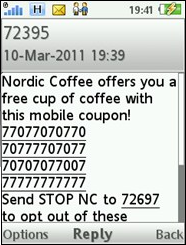
\includegraphics{mcode}
    \caption{Mcode contendo um cupão}
    \label{fig:mcode}
  \end{center}
\end{figure}

\section{Resumo}

O uso de telemóveis em sistemas de transporte público está a aumentar. Os operadores começaram por implementar funcionalidades básicas, como por exemplo o envio de mensagens SMS para consulta de informação, e agora começam a evoluir para processos mais complexos como a compra de títulos de viagem ou até o cálculo automático do preço baseado no percurso efetuado.
\\Com a evolução dos telemóveis e a adição de tecnologias como NFC, adicionar as referidas funcionalidades torna-se mais fácil e viável. Os bilhetes podem ser comprados, descarregados e acedidos através do telemóvel e validados com um simples toque num leitor com tecnologia NFC, emitindo automaticamente uma confirmação. São já várias as redes de transporte a efetuar testes com sistemas de bilhética móvel, ou seja, deixando de parte os cartões físicos e passando todo o processo a ser realizado no dispositivo móvel.
\\Para além disso podem usar-se outras funcionalidades do telemóvel, como por exemplo o ecrã para visualização de bilhetes virtuais, o GPS para determinar a posição atual do passageiro, navegador \textit{web}, câmara, som, etc., para fornecer serviços adicionais aos passageiros, melhorando a experiência de viagem dos passageiros. Partindo desta premissa, o modelo tradicional de serviços de transporte é melhorado com acesso a informação de trânsito e horários em tempo real, possibilidade de consultar instantaneamente o saldo de viagens, planear de forma interativa uma viagem, partilhar opiniões e trajetos com outros passageiros, entre outras possíveis funcionalidades.\cite{Nunes2011}
\\Os telemóveis possuem várias características que os tornam únicos e adequados para serem usados para pagamentos e proporcionarem serviços adicionais: estão ligados à rede constantemente, possuem interfaces de som e texto familiares e fáceis de usar, permitem um acesso a informação em qualquer altura em qualquer lugar, as aplicações são fáceis de descarregar e instalar.
\\Comparando os telemóveis com bilhetes magnéticos no contexto dos transportes públicos, os telemóveis permitem um acesso remoto e ubíquo a serviços de pagamento, eliminando assim a necessidade de esperar numa fila e a necessidade de pagar em dinheiro. Isto é especialmente importante em certas situações em que o passageiro não dispõe de muito tempo disponível antes de iniciar a sua viagem ou não possui dinheiro consigo para efetuar o pagamento.\cite{Mallat2007}
\\Um outro fator importante é o facto de ser menos provável perder o telemóvel do que um bilhete e vários estudos mostram que é menos provável as pessoas saírem de casa sem do telemóvel do que sem a carteira. Adicionalmente, bilhetes em papel acabam por se estragar com o uso intensivo e necessitam de ser substituídos com frequência, o que faz dos bilhetes móveis mais robustos e convenientes, para além de serem uma melhor solução a nível ambiental.
\\Os telemóveis possuem também vantagens em comparação com os cartões sem contacto. Ao contrário destes, o telemóvel pode suportar mais do que um título diferente de mais do que um operador de transportes, enquanto os cartões sem contacto, por norma, apenas permitem um tipo de bilhete, obrigado o passageiro a carregar consigo uma série de cartões diferentes. Isto faz com que, numa carteira com vários cartões, seja necessário retirar o cartão desejado antes de o apresentar à máquina de leitura. Caso contrário, provavelmente não será possível ler o cartão ou será validado um cartão que não o desejado. Em adição a isso, os passageiros podem gerir os seus cartões e bilhetes em qualquer altura em qualquer lugar. Por exemplo, as assinaturas mensais podem ser renovadas sem necessidade de esperar em filas.\cite{NFCForum2011}
\\Por fim, com a gestão feita diretamente no telemóvel do passageiro, é possível aos operadores de transportes públicos interagir com os seus passageiros fazendo sugestões baseadas no perfil de utilização ou oferecer descontos especiais ou pontos de lealdade.\cite{Ferreira2012}